%\documentclass[pdftex]{beamer}
%\documentclass[notes=show]{beamer}
%\documentclass[xcolor=dvipsnames]{beamer}
\documentclass[notes=show,beamer,compress]{beamer}

\usepackage{amssymb}
\usepackage{latexsym}
\usepackage{amsfonts}
\usepackage{amsmath}
\usepackage[absolute,overlay]{textpos}
\usepackage[english]{babel}
\usepackage[latin1]{inputenc}
%\usepackage{times}
\usepackage[T1]{fontenc}
\usepackage{tikz}
\usetikzlibrary{arrows,positioning} 
\usepackage{graphicx}
\usepackage{bigstrut}
\usepackage{bbm}
\usepackage{mathrsfs}
\usepackage{epsfig}
\usepackage{array}
%\usepackage{natbib}

\tikzstyle{arrow} = [thick,->,>=stealth]

\mode<presentation> {
%\usetheme[left,width=1.7cm]{Berkeley}
%\usetheme{default}
\usetheme{Boadilla}
  \usecolortheme[RGB={103,102,204}]{structure}
%\usecolortheme{dove}
  \useoutertheme{infolines}
  \setbeamercovered{transparent}
 }

%\renewcommand{\familydefault}{cmss}
%\renewcommand{\mathrm}{\mathsf}
%\renewcommand{\textrm}{\textsf}
%\usefonttheme{serif}
\newcommand{\X}{{\mathbf{X}}}
\newcommand{\x}{{\mathbf{x}}}
\newcommand{\E}{\mathsf{E}}
\newcommand{\V}{\mathsf{Var}}


    %%%%%%%%%%%%%%%%%%%%%%%%%%%%%%%%%%%%%%%%%%%%%%%%%%%%%%%%%%%%%%%%%%%%%%%%%%%%%%
    %         Neue Kommandos f�r fette Mathebuchstaben innerhalb von Formeln     %
    %%%%%%%%%%%%%%%%%%%%%%%%%%%%%%%%%%%%%%%%%%%%%%%%%%%%%%%%%%%%%%%%%%%%%%%%%%%%%%
    \newcommand{\bom}{\boldmath}
    \newcommand{\ubom}{\unboldmath}
    \newcommand{\mb}{\mathbf}

    \newcommand{\fmalpha}{\mbox{\bom${\alpha}$}}               %Fettes alpha
    \newcommand{\fmbeta}{\mbox{\bom${\beta}$}}                 %Fettes beta
    \newcommand{\fmgamma}{\mbox{\bom${\gamma}$}}               %Fettes gamma
    \newcommand{\fmdelta}{\mbox{\bom${\delta}$}}               %Fettes delta
    \newcommand{\fmepsilon}{\mbox{\bom${\epsilon}$}}           %Fettes epsilon
    \newcommand{\fmvarepsilon}{\mbox{\bom${\varepsilon}$}}     %Fettes varepsilon
    \newcommand{\fmzeta}{\mbox{\bom${\zeta}$}}                 %Fettes zeta
    \newcommand{\fmeta}{\mbox{\bom${\eta}$}}                   %Fettes eta
    \newcommand{\fmta}{\mbox{\bom${\theta}$}}                  %Fettes theta (ta)
    \newcommand{\fmvarta}{\mbox{\bom${\vartheta}$}}         	 %Fettes vartheta (ta)
    \newcommand{\fmiota}{\mbox{\bom${\iota}$}}                 %Fettes iota
    \newcommand{\fmkappa}{\mbox{\bom${\kappa}$}}               %Fettes kappa
    \newcommand{\fmla}{\mbox{\bom${\la}$}}                     %Fettes lambda (la)
    \newcommand{\fmmu}{\mbox{\bom${\mu}$}}                     %Fettes mu
    \newcommand{\fmnu}{\mbox{\bom${\nu}$}}                     %Fettes nu
    \newcommand{\fmxi}{\mbox{\bom${\xi}$}}                     %Fettes xi
    \newcommand{\fmo}{\mbox{\bom${\o}$}}                       %Fettes o
    \newcommand{\fmpi}{\mbox{\bom${\pi}$}}                     %Fettes pi
    \newcommand{\fmvarpi}{\mbox{\bom${\varpi}$}}               %Fettes varpi
    \newcommand{\fmrho}{\mbox{\bom${\rho}$}}                   %Fettes rho
    \newcommand{\fmvarrho}{\mbox{\bom${\varrho}$}}             %Fettes varrho
    \newcommand{\fmsigma}{\mbox{\bom${\sigma}$}}               %Fettes sigma
    \newcommand{\fmvarsigma}{\mbox{\bom${\varsigma}$}}         %Fettes varsigma
    \newcommand{\fmtau}{\mbox{\bom${\tau}$}}                   %Fettes tau
    \newcommand{\fmupsilon}{\mbox{\bom${\upsilon}$}}           %Fettes upsilon
    \newcommand{\fmphi}{\mbox{\bom${\phi}$}}                   %Fettes phi
    \newcommand{\fmvarphi}{\mbox{\bom${\varphi}$}}             %Fettes varphi
    \newcommand{\fmchi}{\mbox{\bom${\chi}$}}                   %Fettes chi
    \newcommand{\fmpsi}{\mbox{\bom${\psi}$}}                   %Fettes psi
    \newcommand{\fmomega}{\mbox{\bom${\omega}$}}               %Fettes omega
    \newcommand{\fmimath}{\mbox{\bom${\imath}$}}               %Fettes imath

     \newcommand{\fmv}{\mathnormal{v}}               %v
      \newcommand{\fmu}{\mathnormal{u}}               %v
      \newcommand{\fme}{\mathnormal{e}}               %v


\setbeamercolor{bibliography entry title}{fg=black}
\setbeamercolor{bibliography entry author}{fg=black}
\setbeamercolor{subsection in toc}{fg=structure}
\setbeamercolor{palette primary}{bg=structure, fg=white}
%\setbeamercolor{palette secondary}{bg=structure, fg=black}
%\setbeamercolor{palette tertiary}{bg=structure, fg=black}
\setbeamercolor{caption name}{fg=black} \setbeamersize{text margin
left=.8cm} \setbeamersize{text margin right=1cm}
\hypersetup{linkbordercolor={1 0 0}} \setbeamertemplate{navigation
symbols}{} \setbeamertemplate{headline}[default]

\setbeamertemplate{enumerate items}[default]

\newcounter{transfct}
\newcounter{begbs}
\newcounter{endbs}
\title[Panel Data Models]{Econometrics 2}
\subtitle{Panel Data Models}
\author[Lychagin \& Mu\c{c}o]{Sergey Lychagin}
\institute[CEU]{CEU}
\date{Winter 2020}


\AtBeginSection[] {
  \begin{frame}<handout:0>
    \frametitle{TOC}
    \tableofcontents[currentsection]
  \end{frame}
}

%\AtBeginSubsection[] {
%  \begin{frame}<beamer>
%   \frametitle{Outline}
%    \tableofcontents[currentsection,currentsubsection]
%  \end{frame}
%}

%\beamerdefaultoverlayspecification{<+->}

\begin{document}

\frame{\titlepage}

\begin{frame}
\frametitle{Upcoming topics}

\begin{itemize}
  \item Panel data, first differences, fixed effects estimator
  \item Difference-in-Differences designs

   \end{itemize}
\end{frame}


\begin{frame}
\frametitle{Omitted variables formula}

If the \emph{true} model is
\[ Y_i = X_i'\beta + \varepsilon_i \]
and $E\left[X_i  \varepsilon_i \right]\neq 0$, then we know that the population regression gives 
\begin{eqnarray*}
 \beta^{OLS} &=& \beta + \pi \\
         \pi &=& E\left[X_i  X_i' \right]^{-1} E\left[X_i  \varepsilon_i \right]\
\end{eqnarray*}
$\pi$ is the vector of regression coefficients when we regress $\varepsilon_i$ on $X_i$ (which is not practically possible)

\end{frame}


\begin{frame}
\frametitle{First Approach: observed covariates $Z$}

True causal model
\[ Y_i = X_i'\beta + \varepsilon_i \]
in which
\begin{itemize}
  \item We know that $Y_i$ depends on observed $X_i$'s and unobserved $\varepsilon_i$
  \item Not all the observed covariates $Z$ belong in the model 
  \item We know something about $\varepsilon_i$, e.g. $\varepsilon_i=u_i + w_i$, where $w_i$ --- idiosyncratic shock (i.e., unrelated to $X$).
 \end{itemize}
 
 Possible Approaches
 
 \begin{itemize}
  \item Use the $Z's$ to ''control for'' $u_i$ (proxy)
  \item  Use the $Z's$ to get the part $X_i$ that is unrelated to $u_i$ (IV)
 \end{itemize}
\end{frame}


\begin{frame}
\frametitle{Second Approach: Panel data}

We make assumptions on the nature of $\varepsilon_i$ and how it is related to $X_i$
\bigskip

Second approach: Panel data setting with units $i=1, ..., N$ and periods  $t=1, ..., T$
\begin{eqnarray*}
 Y_{it} &=& X_{it}'\beta + \varepsilon_{it}\\
         \varepsilon_{it} &=& u_i + w_{it} \\
         E\left[X_{it} \varepsilon_{it}\right] &=& E\left[X_{it} u_{i}\right]+ E\left[X_{it} w_{it}\right]
\end{eqnarray*}
It might be reasonable to assume $ E\left[X_{it} w_{it}\right]=0$, the idiosyncratic part of the error term is not correlated with observable $X$.\\\bigskip

Example (\emph{pre-determined covariates}): $Y_{it}$ firm $i$'s log of output at $t$, $X_{it}$ --- capital, labor. If inputs are hired at $t-1$ and $w_{it}$ is unexpected, $E[X_{it}w_{it}]=0$.

\end{frame}


\begin{frame}{Varieties of data}
	\begin{itemize}
				\item{Repeated cross section
			\begin{itemize}
				\item{We draw a sample of individuals, \textbf{independently for each $t$}. We do not track individuals over time}
		\end{itemize}}
		\item{Panel data
			\begin{itemize}
				\item{There is a population at $t=1,..,T$,}
				\item{We draw a sample of individuals}
				\item{Every individual comes with a whole history of $(Y_{it}, x_{it})$}
			\end{itemize}}

		\item{Balanced panel: no holes; we have data for all $(i, t)$ pairs.}
		\item{Unbalanced panel: there are holes (due to random or non-random selection).}
	\end{itemize}
\end{frame}

\begin{frame}
\frametitle{Repeated Cross Sectional Data}

Cross-sectional data
\begin {itemize}
\item Random sample of the population, independent observations
\item Example: German Labor Force Survey (Mikrozensus), survey of 1\% of German households: about 370,000 households with 870,000 individuals
\end{itemize}
Many cross-sectional surveys are repeated over time

\end{frame}

\begin{frame}
\frametitle{Repeated Cross Sectional Data}

Example: returns to education over time

\begin {itemize}
\item cross section $t=2000$
\[ log(w_i) = \alpha + \beta educ_i + \varepsilon_i \]
\item pooled cross sections $t=2000, 2005$
\begin{eqnarray*} log(w_{it}) &=& \alpha_0 +  \alpha_1 y05  + \beta_0 edu_{it} + \beta_1 edu_{it}\times{}y05 + \varepsilon_{it} 
\end{eqnarray*}
\item pooled cross sections $t=2000, 2005, 2010$
\begin{eqnarray*} log(w_{it}) &=& \alpha_0 +  \alpha_1 y05  +  \alpha_2 y10 \\
&+& \beta_0 edu_{it} + \beta_1 edu_{it} *y05 + \beta_2 edu_{it} *y10 + \varepsilon_{it} 
\end{eqnarray*}
\end{itemize}
As long as $E[X_{it}\varepsilon_{it}]=0$, OLS gives the causal effect.
\end{frame}

%slide 7

\begin{frame}
\frametitle{Panel Data}


\begin {itemize}
\item Repeated observations of the same unit

\item  $i=1\ldots N$, can be countries, firms, regions
\item $t= 1\ldots T$ denotes time

\item \textbf{Example 1}: Financial statements of Hungarian firms

\begin {itemize}
\item Collected by the State Tax Authority
\item All double-entry bookkeeping firms in Hungary (150-400 thousand, depending on year).
\end{itemize}

\item \textbf{Example 2}:

\begin {itemize}
\item \textit{i}: family, and \textit{t}: twin 1 or 2
\end{itemize}

\item We consider applications where $N$ is large and $T$ small (``short panels'')

\end{itemize}
\end{frame}


\begin{frame}
\frametitle{Outline}

\begin{itemize}
  \item Case 1: $T=2$
  \item Case 2: $T>2$
  \item Fixed effects estimation
\end{itemize}
\end{frame}



% slide 8

\begin{frame}
\frametitle{Case 1: $T=2$}
\begin{itemize}
\item Example: twin data, $i$ -- family, $t$ -- child.
\item Fixed Effects Model:
\[\begin{array}{cc}
  Y_{it}=  X_{it} \beta + u_i + w_{it}
\end{array}
\]
\item $u_i$ unobserved effect, fixed effect, or unobserved heteregeneity
\item $w_{it}$ idiosyncratic error

\item Estimate with OLS - \emph{Pooled Model}:
\begin{eqnarray*}
  Y_{it}&=& \beta X_{it}  + \varepsilon_{it}\\
  \varepsilon_{it} &=&  u_i + w_{it},  \text{(composite error)}
\end{eqnarray*}
\item If we estimate this model with OLS, we need $E\left(Xu\right)=0$ to recover the causal effect.
\item This implies the assumption that  $u_i$ is uncorrelated with $X_{it}$.
\item{E.g., $Y_{it}$ -- wage, $X_{it}$ -- education, $u_i$ -- genetic factors. Is $X_{it}$ unrelated to $u_i$?}
\end{itemize}
\end{frame}


% slide 9

\begin{frame}
\frametitle{Panel Estimation}

Individual effect $u_i$ causes trouble. Three solutions:
\begin{enumerate}
	\item Control for it: include a dummy for each $i$ in the model.
	\begin{itemize}
	\item  LS dummy variable estimator
	\item Large number of regressors: dimension of  $X$ is $ NT\times (k+N) $
	\item computationally demanding
	\end {itemize}
	\item Get rid of it by first differencing. Then, apply OLS:
\begin{eqnarray*}
Y_{i2}-Y_{i1} &=& \left(X_{i2}-X_{i1}\right)\beta + \left(w_{i2}-w_{i1}\right)\\
\Delta Y_{it} &=& \Delta X_{it} \beta   + \Delta w_{it}
\end{eqnarray*}
\item Get rid of it by de-meaning:
\begin{eqnarray*}
	Y_{it}-\overline{Y}_i &=& \left(X_{it}-\overline{X}_i\right)\beta + \left(w_{it}-\overline{w}_i\right)\\
	\widetilde{Y}_{it} &=& \widetilde{X}_{it} \beta   + \widetilde{w}_{it}
\end{eqnarray*}
\end{enumerate}
If $T=2$, the results are numerically identical.
\end{frame}




% slide 10


\begin{frame}
\frametitle{Estimation assumptions in the FD model}
     \begin {itemize}

     \item $\left(X_{i2}-X_{i1}\right)$ has to be uncorrelated with $\left(w_{i2}-w_{i1}\right)$
     \item This holds if $w_{it}$ is uncorrelated with both  $X_{i1}$ and $X_{i2}$: \emph{Strict Exogeneity} (strong exogeneity in some textbooks)
	 \item $\left(X_{i2}-X_{i1}\right)$ must have some variation in $i$: e.g. not all twins have same level of schooling.
      \end {itemize}
Example: Control for ability bias in return to education.
\begin{eqnarray*}
Y_{it}& = &\alpha + X_{it}\beta + S_{it}\delta+ A_i + \epsilon_{it} \\
\Delta Y_{it} &= & \Delta X_{it}\beta + \Delta S_{it}\delta+  \Delta \epsilon_{it}
\end{eqnarray*}
 Usually there is no variation in $\Delta S_{it}$ in a sample of adult workers: cannot estimate $\delta$ with precision/at all.

\end{frame}


% Slide 11

\begin{frame}
\frametitle{Case 2: $T>2$}

\begin{eqnarray*}
Y_{it} &=&  X_{it}\beta + \delta_t +  u_i+ w_{it}
\end{eqnarray*}

\emph{First differenced} model with $(T-1)$ equations:
\begin{eqnarray*}
Y_{it}-Y_{it-1} &= & (X_{it}-X_{it-1})\beta + ( \delta_t - \delta_{t-1}) + (w_{it}-w_{it-1})
\end{eqnarray*}
\begin {itemize}
\item $\delta_t$ --- time-varying intercepts.
\item Condition to uncover the causal effect if we estimate the FD model with OLS: $E(\Delta{}X_{it} \Delta{}w_{it})=0$

\item holds if $Cov( X_{it},w_{is})=0$,  for all $t,s$ : \emph{Strict Exogeneity}
\end {itemize}
\end{frame}


\begin{frame}
\frametitle{Strict exogeneity assumption}
\begin {itemize}
\item Example: dynamic model
\begin{eqnarray*}
Y_{it} &=&  Y_{it-1} \beta + u_i + w_{it} \\
Y_{it}-Y_{it-1} &= & (Y_{it-1}-Y_{it-2})\beta+ (w_{it}-w_{it-1})
\end{eqnarray*}
Here: $(w_{it}-w_{it-1})$ is correlated with  $(Y_{it-1}-Y_{it-2})$ by construction
\item Strict exogeneity also rules out cases where future explanatory variables react to changes in the idiosyncratic errors.\\\medskip
Example: firm $i$ discovers its productivity improved (high $w_{it}$) $\Longrightarrow$ $i$ hires more workers tomorrow ($X_{it+1}\uparrow$).
\end {itemize}
\end{frame}



\begin{frame}{Remarks on FD.}
\begin{itemize}
\item{Always, always include time dummies. Example:
	\begin{itemize}
		\item{$Y_{it}$ is deflated revenue of firm $i$, $X_{it}$ is deflated capital stock (in logs).}
		\item{Imperfect deflation: suppose $Y_{it}$ and $X_{ik}$ both have upward trends due to this --- \textbf{coincidental trends!}}
		\item{Coefficient on $\Delta{X}_{it}$ will pick this up even if capital does not have effect on output.}
	\end{itemize}}
\item{Differencing may amplify measurement error. Example: coef. on capital often too low in production function estimates. Why?
\begin{itemize}
	\item{Differencing wipes out cross-sectional variation in the data.}
	\item{If measurement error is independent across $t$, it's variation stays the same.}
	\item{$\Rightarrow$ Relative variation in error grows $\Rightarrow$ attenuation bias $\uparrow$.}
\end{itemize}}
\end{itemize}
\end{frame}

% slide 12

\begin{frame}
\frametitle{Fixed Effects Estimation}
FE = OLS with individual dummies, but less computationally expensive.\\
Use OLS to estimate the \emph{time demeaned} model:
\begin{eqnarray*}
  Y_{it}-\bar{Y}_{i} &=& ( X_{it}-\bar{X}_{i}) \beta +( \delta_t-\bar{\delta}) +(w_{it}- \bar{w}_{i})
\end{eqnarray*}
also called within transformation or fixed-effects (FE) transformation

\begin{itemize}
\item All time constant variables drop out of the fixed effects  model
\item \emph{Strict exogeneity} assumption necessary to get the causal effect
\item Fixed effects and FD estimators are generally different for $t>2$
\item To compute correct standard errors use FE procedures (more on this later)
\end{itemize}
\end{frame}

%slide 13

\begin{frame}
\frametitle{Fixed effects estimation}

Estimation of $\hat{u_{i}}$, $i=1,...,N$
\begin{eqnarray*}
\hat{u}_{i}=\bar{Y_i}-\bar{X_i}\hat{\beta}-\bar{\delta}
\end{eqnarray*}

\begin{itemize}
\item We think of a situation where $T$ is fixed and $N$ increases to do statistical inference.
\item For every $i$ that is added to the sample, we would get an additional estimate for $u_i$.
\item In this model estimates $\hat{u}_{i}$ are not meaningful (inconsistent).
\end{itemize}
\end{frame}


\begin{frame}{Why does OLS work and how to compute std. errors?}

FD and FE estimators are just OLS on transformed data. Can't one just use standard errors from the OLS output?\\\bigskip

Not a good idea: OLS assumes $\Delta{}X_{it}$ and $\Delta{}X_{it+1}$ are independent. But they are not --- transforming the data creates \emph{serial correlation}.

\end{frame}

\begin{frame}{Recall theory behind OLS}
Consider a model with one variable:
\begin{equation*}
	Y_i = \beta_0 + \beta_1X_i + \varepsilon_i, \quad E[\varepsilon_i|X_i]=0
\end{equation*}
OLS
\begin{equation*}
	\widehat\beta_1 = \frac{\frac{1}{N}\sum_i(X_i - \bar{X})Y_i}{\frac{1}{N}\sum_i(X_i - \bar{X})^2} = \beta_1 + \frac{\frac{1}{N}\sum_i(X_i - \bar{X})\varepsilon_i}{\frac{1}{N}\sum_i(X_i - \bar{X})^2}
\end{equation*}
CLT: $\frac{\frac{1}{N}\sum_i(X_i - \bar{X})\varepsilon_i - E[X\varepsilon]}{\sqrt{N}} \to N[0, V]$, where $V = E[(X-E[X])^2\varepsilon^2]$\\
LLN: $\frac{1}{N}\sum_i(X_i - \bar{X})^2 \to \sigma^2_X$.\\\bigskip

In the limit, standard error of $\widehat\beta_1$ is $\sigma_{\widehat\beta_1} = \sqrt{V}/\sigma^2_X$. We know neither $V$, nor $\sigma_X$, need to estimate both.
\end{frame}


\begin{frame}{Homoskedastic errors}
Suppose $E[\varepsilon^2|X] = \sigma_\varepsilon^2$. Estimating $V$ and $\sigma_X$ in $\sigma_{\widehat\beta_1} = \sqrt{V}/\sigma^2_X$:
\begin{enumerate}
	\item{$\widehat\sigma_X = \sqrt{\frac{1}{N}\sum_i(X_i-\bar{X})}$}
	\item{$V = E[(X-E[X])^2\varepsilon^2] = E[(X-E[X])^2]\sigma_\varepsilon^2$:
		\begin{align*}
			\widehat{V} = \frac{1}{N}\sum_i(X_i -\bar{X})^2\widehat{\sigma}_\varepsilon^2, \quad \widehat{\sigma}_\varepsilon^2 = \frac{1}{N}\sum_i\widehat{\varepsilon}_i^2
		\end{align*}
	}

\end{enumerate}

This is what you get if you run 
\begin{center}
	\texttt{regress y x} 
\end{center}
without any extra options

\end{frame}


\begin{frame}{Heteroskedasticity-robust errors}
Suppose $E[\varepsilon^2|X] \neq{const}$:
\begin{enumerate}
	\item{$\widehat{\sigma}_X^2$ --- same as before}
	\item{Estimating $V = E[(X-E[X])^2\varepsilon^2]$
		\begin{align*}
		\widehat{V} = \frac{1}{N}\sum_i(X_i -\bar{X})^2\widehat{\varepsilon}_i^2
		\end{align*}
	}
\end{enumerate}

This is what you get if you run 
\begin{center}
	\texttt{regress y x, robust} 
\end{center}
\end{frame}

\begin{frame}{Dealing with serial correlation}
So, what's the deal with serial correlation?
\begin{itemize}
	\item{}LLN and CLT work if $(X_i, Y_i)$ is independent of $(X_j, Y_j)$. 
	\item{}When we use FD we run $\Delta{}Y_{it}$ on $\Delta{}X_{it}$. But $\Delta{}Y_{it}$ is correlated with $\Delta{}Y_{it-1}$!
\end{itemize}
Would OLS on transformed data still work? Standard errors?

\end{frame}


\begin{frame}{Dealing with serial correlation: clustering}
Suppose we run FD (balanced panel, zero time effects):
\begin{equation*}
\Delta{}Y_{it} = \beta_1\Delta{}X_{it} + \Delta{}w_{it}, \quad E[w_{it}|X_{is}]=0 \text{ for all $s,t$}
\end{equation*}
\begin{equation*}
\widehat\beta_1 = \beta_1 + \frac{\frac{1}{NT}\sum_i\sum_t\Delta{}X_{it}\Delta w_{it}}{\frac{1}{NT}\sum_i\sum_t(\Delta{}X_{it})^2}
\end{equation*}
Cluster observations by cross-sectional unit. For instance, in the numerator:
\begin{align*}
\frac{1}{N}\sum_i\underbrace{\left[\frac{1}{T}\sum_t\underbrace{\Delta{}X_{it}\Delta{}w_{it}}_{\text{not i.i.d.}}\right]}_{i.i.d.}
\end{align*}
Quantities in brackets are i.i.d.: trajectories of $(X_i, Y_i)$ are sampled randomly. Terms in the inner $\sum$ are correlated with one another.

\end{frame}


\begin{frame}{Dealing with serial correlation: clustering}
So we can use CLT, but apply it to clusters rather than observations. CLT:
\begin{align*}
\frac{1}{N}\sum_i\left[\frac{1}{T}\sum_t\Delta{}X_{it}\Delta w_{it}\right]\to{}N[0, V], \quad V = Var\left[\frac{1}{T}\sum_t\Delta{}X_{it}\Delta w_{it}\right]
\end{align*}
Estimating $V$:
\begin{align*}
	\widehat{V} = \frac{1}{N}\sum_i\left[\frac{1}{T}\sum_t\Delta{}X_{it}\widehat{\Delta w}_{it}\right]^2
\end{align*}
Standard error for $\widehat\beta_1$: $\widehat{\sigma}_{\widehat{\beta}_1} = \sqrt{\widehat{V}}/\widehat{\sigma}_{\Delta{}X}^2$
This is what you get if you run
\begin{center}\texttt{
	regress y x, vce(cluster i)}
\end{center}

\end{frame}

\begin{frame}{Stata tips}
\begin{itemize}
	\item{
	Set up your panel data before use:
\begin{center}
	\texttt{xtset i t}
\end{center}
where \texttt{i} -- cross-sectional id, \texttt{t} -- time id.}
	\item{First difference of $X$, $\Delta{}X_{it}$: \texttt{D.X}}
	\item{First lag, $X_{it-1}$: \texttt{L.X}}
	\item{Second lag, $X_{it-2}$: \texttt{L2.X}}
\end{itemize}
FD estimator w/o time dummies:
\begin{center}
\texttt{regress D.Y D.X, vce(cluster i)}\\\smallskip
\end{center}
FE estimator:
\begin{center}
\texttt{xtreg Y X, fe vce(cluster i)}
\end{center}
Don't forget to use the ``fe'' option!
\end{frame}

\begin{frame}{Clusters and sample size}
	Standard tests and confidence intervals are precise when the sample is large enough for the CLT to kick in. Otherwise $\widehat\beta - \beta \not\approx$ normal r.v.\\\medskip
	
	\begin{block}{Typical faulty reasoning}
		\itshape
		``I run GDP on interest rate for the 15 post-Soviet countries. A sample of 15 observations is clearly too small. However, I use a 20-year panel, which gives me 300 observations. I heard that OLS is fairly reliable if the number of observations is 100 or higher''
	\end{block}
	Remember: in the panel setting CLT is applied to \textbf{countries} (outer sum) rather than country-year pairs (inner sum):
	\begin{align*}
	\frac{1}{N}\sum_i\left[\frac{1}{T}\sum_t\Delta{}X_{it}\Delta w_{it}\right]\to{}N[0, V]
	\end{align*}
	Relevant sample size is still $N=15$.
\end{frame}


% slide 14

\begin{frame}
\frametitle{Application: Return to computer use}

Stylized fact: workers who use computers earn more. Interpretation is hard:
\begin{center}
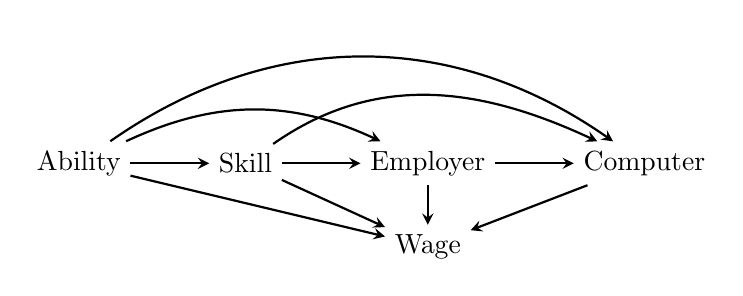
\begin{tikzpicture}[node distance=1cm, auto,]

	\node(ability) {Ability};
	\node[right= of ability](skill) {Skill};
	\node[right= of skill](firm) {Employer};
	\node[right= of firm](computer) {Computer};
	\node[below=0.5cm of firm](wage){Wage};
	
	\draw[arrow] (ability) -> (skill);
	\draw[arrow] (skill) -> (firm);
	\draw[arrow] (firm) -> (computer);
	\draw[arrow] (ability) to[out=35, in=145](computer);
	\draw[arrow] (ability) to[out=25, in=155](firm);
	\draw[arrow] (skill) to[out=35, in=155](computer);
	\draw[arrow] (ability) -> (wage);
	\draw[arrow] (skill) -> (wage);
	\draw[arrow] (firm) -> (wage);
	\draw[arrow] (computer) -> (wage);
	
\end{tikzpicture}
\end{center}
\begin{itemize}
	\item Data: French Labor Force Survey, rotating panel of 9000 individuals 1991-1993. $T=3$, $N=9000$.
	\item Computer use supplement in 1993.
	\item 905 individuals change status from non-users to computer users in the sample.
\end{itemize}
\begin{equation*}
ln(w_{it})=\rho Comp_{it} + X_{it} \beta + \delta_t + F_{j(i,t)} + A_i +\epsilon_{it}
\end{equation*}
\end{frame}


\frame{ \frametitle{}
\begin{center}
\begin{figure}[t]
\includegraphics[width=0.6\linewidth]{"graphs/ent_tab4"}
\end{figure}
\end{center}
 }

\frame{ \frametitle{}
\begin{center}
\begin{figure}[t]
\includegraphics[width=0.8\linewidth]{"graphs/ent_tab5"}
\end{figure}
\end{center}
 }

\begin{frame}{FE vs FD?}
	\begin{itemize}
		\item{FD discards many observations if the dataset has many holes.}
		\item{FE may be less sensitive to timing misspecification than FD
			\begin{itemize}
				\item{Consider $\log{WAGE} = \beta_0 + \beta_1YEARS\_EDUC + \varepsilon$ }
				\item{On years when $YEARS\_EDUC$ grows, $WAGE$ is zero or close to zero (school/college) and vice versa.}
				\item{Plot FD, demeaned data.}
			\end{itemize}}
		\item{FD: Strict exogeneity sufficient, but not necessary.}
	\end{itemize}
	Try both.
\end{frame}

\begin{frame}{Notes on FD and FE}
Unbalanced panel? Beware of sample selection
\begin{itemize}
	\item{Selection on observables is not an issue, as usual.}
	\item{Selection on individual intercept is okay (e.g., lower ability workers having more holes in the data).}
	\item{Selection on time-varying unobservables is still a problem.}
\end{itemize}
The effect is identified off switchers (e.g., no computer $\to$ computer and vice versa). 
\begin{itemize}
	\item{No way to tease out the effect of time-invariant variables (e.g., gender, race).}
	\item{Selection on treatment effects! In theory, switchers are almost indifferent between treatment and no treatment.}
\end{itemize}
Think hard what makes people switch. Why is this unrelated to the effect of interest?
\end{frame}

\begin{frame}{Random effects estimator?}
	Some of you have heard about the random effects estimator.
	\begin{itemize}
		\item{More efficient (tighter confidence intervals) than FE.}
		\item{But requires stronger assumptions.}
		\item{A dealbreaker: $u_i$ cannot correlate with $X_{it}$. E.g., computer use is independent of ability (!)}
		\item{Hence, RE is never used for causal inference.}
	\end{itemize}
\end{frame}

\begin{frame}{Dynamic models?}
A model with lags of outcome on the RHS. For instance, think of firm-level employment ($i$ -- firm, $t$ --year):
\begin{multline*}
	\log{EMPLOYMENT_{it}} = \rho\log{EMPLOYMENT_{it-1}} + \beta{}X_{it} + u_i + w_{it}
\end{multline*}
$X_{it}$ --- gov't grants, access to credit. Lag: adjusting employment is subject to frictions.\\\medskip

Cannot use FD or FE: strict exogeneity is violated ---$w_{it}$ is correlated with the RHS at $t+1$.
\end{frame}

\begin{frame}{Dynamic models? Arellano-Bond estimators.}
Take differences:
\begin{multline*}
\Delta\log{EMPLOYMENT_{it}} = \rho\Delta\log{EMPLOYMENT_{it-1}} + \beta{}\Delta{}X_{it} + \Delta{}w_{it}
\end{multline*}
Fixed effect $u_i$ is gone. Next step --- use lagged levels of $X_{it}$ to instrument for $\log{EMPLOYMENT_{it-1}}$ and $\Delta{}X_{it}$. Intuition?
\begin{itemize}
	\item{$X_{it}$ fluctuates around some ``steady state''. If $X_{it-1}$ is too high, $\Delta{}X_{it}$ is likely to be negative and vice versa.}
	\item{$\log{EMPLOYMENT_{it-1}}$ is partly driven by $X_{it-1}, X_{it-2}, \dots$. Generous gov't support in the past $\to$ more workers at $t-1$.}
\end{itemize}
Need contemporaneous and past exogeneity only: ``future shocks do not affect past choices''
\begin{equation*}
	E[w_{it}|X_{it}, X_{it-1}, \dots] = 0.
\end{equation*}
$X_{it+1}$ can respond to $w_{it}$, strict exogeneity is not necessary.
\end{frame}

\begin{frame}{Arellano-Bond estimators. Notes.}
\begin{itemize}
	\item{Many ways to implement --- what lags to include? Instrument with past levels or past differences or both?}
	\item{Degrees of freedom $\uparrow$ $\Rightarrow$ trust in estimates $\downarrow$. Fishing for significance, convenient results?}
	\item{Non-transparent identification --- most applications rely on handwaving rather than carefully exploited natural experiments.}
	\item{But sometimes this is the best you can do (quick and dirty policy research).}
\end{itemize}
\end{frame}

%
%
%%slide 15
%
%\begin{frame}
%\frametitle{Unbalanced Panels}
%\begin{itemize}
%\item Missing time periods for same cross sectional units
%\item $T_{i}$ number of periods for unit \textit{i}
%\item Use those for time de-meaning
%\item Number of observations $T_{1}+\ldots + T_{N}$
%\item Adjust degrees of freedom
%\item Units with only a single time period drop out
%\item Why is the panel unbalanced?
%
%\begin{itemize}
%  \item Individuals refuse to respond? No random event firms going out of business
%  \item Nonrandom sample is subsequent periods
%  \item Attrition correlated with $\epsilon_{it}$
%  \item Selection Problem- biased estimators
%\end{itemize}
%
%\item FE allows attrition to be correlated with $\epsilon_{i}$
%
%
%\end{itemize}
%
%\end{frame}

%
%\begin{frame}
%\frametitle{Generalized Least Squares (GLS)}
%
%Estimation of the error variance matrix $E(uu')$ along with the coefficient vector $\beta$
%\begin{itemize}
%\item needs special assumptions about the error structure, otherwise there are too many parameters
%\item GLS is more efficient, if the assumptions are correct
%\item GLS can be biased, if the assumptions are not correct
%\end{itemize}
%
%\end{frame}
%
%%slide 16
%
%\begin{frame}
%\frametitle{Random effects model}
%
%\begin{equation*}
%Y_{it} = X_{it} \beta + A_i +\epsilon_{it}
%\end{equation*}
%\begin{itemize}
%\item Assume that $A_i$  uncorrelated with $X_i$  in all $t$
%\item \emph{random effects} model
%\item In this case we can estimate the causal effect $\beta$ with OLS
%\begin {enumerate}
%\item Using a simple time period (cross section), disregarding a lot of information.
%\item Pooled OLS regression
%\end {enumerate}
%\end{itemize}
%
%\end{frame}
%
%
%
%
%
%
%%slide 17
%
%\begin{frame}
%\frametitle{Random effects model}
%
%Estimating with pooled OLS
%\begin{eqnarray*}
%Y_{it} &=& X_{it} \beta + A_i + \epsilon_{it} = X_{it} \beta + u_{it} \\
%Cov(u_{it}, u_{is}) &=& Cov( A_i+ \epsilon_{it}, A_i+ \epsilon_{is})\\
%                    &=& Var(A_i)+ Cov( \epsilon_{it}, \epsilon_{is}) \\
%                    &=& \sigma^{2}_{a}	 \\
%Corr(u_{it}, u_{is})&=& \frac{\sigma^{2}_{a}}{\sigma^{2}_{a}+\sigma^{2}_{\epsilon}}\neq0
%\end{eqnarray*}
%
%\begin{itemize}
%\item Serial Correlation in the error term
%
%\begin{eqnarray*}
%E(uu^{'}| X)&=& \sigma^{2}\Omega\neq\sigma^2I,    \nonumber
%\end{eqnarray*}
%
%\item Random effects estimator: Use GLS, exploiting structure of serial correlation and estimate $\hat{\Omega}$
%\end{itemize}
%
%\end{frame}
%
%
%
%%slide 18
%
%\begin{frame}
%\frametitle{Random effects transformation}
%\begin{eqnarray*}
%	\lambda &=& 1-\sqrt{\sigma^{2}_{\epsilon}/(\sigma^{2}_{\epsilon}+T\sigma^{2}_{a})}\nonumber\\
%	0 &\leq& \lambda\leq1\nonumber
%\end{eqnarray*}
%
%
%\begin{itemize}
%\item Transformed Equation:
%\begin{align}
%	Y_{it} -\lambda \bar{Y_{i}}= (X_{it}-\lambda \bar{X_{i}}) \beta + (u_{it}- \lambda \bar{u_{i}})\nonumber
%\end{align}
%\item Quasi-demeaned model
%\item Random effects model subtracts fraction $\lambda$ of time averages
%\item We can include variables that are constant over time
%\item Cost: Assume $A_i$ uncorrelated with all $X$ variables.
%\end{itemize}
%
%\end{frame}
%
%
%
%
%%slide 25
%
%\begin{frame}
%\frametitle{Notes}
%\begin{itemize}
%\item No variables that one constant over time, no constant in the model.
%\item Single $X$
%\begin {itemize}
%\item All observation $i$ for which $X$ is constant over time drop out.
%
%\end {itemize}
%
%\item $\beta$ only identified by ``switchers"
%
%\end{itemize}
%
%\end{frame}
%
%
%
%
%
%
%
%
%
%




\end {document}